
%%pyramid%%%
\begin{frame}{}
    \Large
    \centering
    The langauge of maths is \textbf{proof}.\\ 
    \normalsize 
    % \vspace{10pt}
    \begin{columns}
        \textbf{\null}%place holder
        \begin{column}{.5\textwidth}
            \only<2-3,10->{%
                \begin{itemize}
                    \item<2->[] But what is a proof???
                    \item<10->[] A way to communicate aboslute tRUTHS, through logic.
                \end{itemize}
            %     \begin{itemize}
            % %         
            %     \end{itemize}
            }
            \vspace{20pt}
            \Large \only<11->{If (something is true)}
            \only<12->{then (something else is true)}
        \centering 
            \only<4>{\begin{figure}
                \centering
                
\includegraphics[width =.6\textwidth]{./images_women_in_IT/Georg_Cantor_eyes_smile.png}
                \caption*{Georg Cantor (1845-1918)}
            \end{figure}}
            \only<5>{\begin{figure}
                \centering
                \vspace{20pt}
                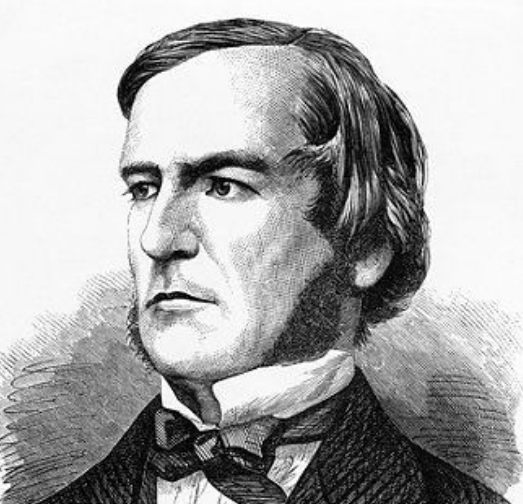
\includegraphics[width =.6\textwidth]{./images_women_in_IT/Boole.png}
                \caption*{George Boole (1815-1864)}
            \end{figure}}
            \only<6-9>{\begin{figure}
                \centering
                \vspace{20pt}
                
\includegraphics[width =.6\textwidth]{./images_women_in_IT/BooleCool.png}
                \caption*{George Boole (1815-1864)}
            \end{figure}}
        \end{column}
        
        %%%%
        \begin{column}{.5\textwidth}
            \vspace{10pt}
            \begin{figure}
                \includegraphics<3>[width=.8\textwidth]{./images_women_in_IT/mathpyramid1.png}
                \includegraphics<4>[width=.8\textwidth]{./images_women_in_IT/mathpyramid2.png}
                \includegraphics<5>[width=.8\textwidth]{./images_women_in_IT/mathpyramid3.png}
                \includegraphics<6>[width=.8\textwidth]{./images_women_in_IT/mathpyramid4.png}
                \includegraphics<7>[width=.8\textwidth]{./images_women_in_IT/binary.png}
                \includegraphics<8>[width=.8\textwidth]{./images_women_in_IT/graphs.png}
                \includegraphics<9-12>[width=.8\textwidth]{./images_women_in_IT/binary.png}
                \includegraphics<13>[width=.9\textwidth]{./images_women_in_IT/code_example.png}
            \end{figure}    
        \end{column}
    \end{columns}
\end{frame}

\begin{frame}[t]
\frametitle{You've all dones this.} 
\large
    \[
        \begin{array}{rcl}
            \onslide<2->{x^2 -2x-15 &=& 0} \\[6pt]
            \onslide<3->{x^2 -5x + 3x -15 &=& 0} \\[6pt]
            \onslide<4->{(x-5)(x+3)&=& 0} \\[6pt]
            \onslide<5->{x&=& 5 \text{ or } -3 } 
        \end{array}
    \]
\end{frame}

\begin{frame}[t]
    \vfill
    \begin{columns}
        \begin{column}{.35\textwidth}
            \begin{itemize}
                \item<2-> Direct proof. 
                \item<3-> Proof by contradiction.
                \item<4-> Proof by induction. 
            \end{itemize}
        \end{column}
        %%%%
        % \begin{column}{.55\textwidth}
        % \end{column}
    \end{columns}
    \vspace{20pt}
    % \centering
    % \only<3>{If \textbf{A} then \textbf{B}}
    % \only<5>{If (\textbf{A} then \textbf{NOT B}), then something absurd, then If \textbf{A} then \textbf{B}}
    % \only<7>{If \textbf{A} for $n$ then \textbf{A} $n+1$, and \textbf{A} for some $n=x$, then \textbf{A} for all $n\geq X$.}
\end{frame}

% \begin{frame}[t]
% \frametitle{You've all dones this.}
% A phone, a phone, and a phone are added to an unknown number of phones. The result is equal to a phone, phone, phone, phone, and phone. 
% \\ \vspace{20pt}
% \Large
% \centering
% \only<2>{\phone, \phone, \& \phone{} are  added to an \framebox{? \phone's}. The result is equal to \phone, \phone, \phone, \phone, \& \phone. }
% \only<3>{$3 \times$ \phone's are  added to an \framebox{? \phone's}. \\The result is equal to $5 \times$ \phone's. }
% \only<4>{$3 \times $ \phone's $+$ \framebox{? \phone's} $ = 5 \times $\phone's. }
% \only<5>{$3  +$ \framebox{? \phone's} $ = 5$. }
% \only<6->{$3 + x = 5$}
% \vspace{10pt}
% \only<7>{\\ $\Rightarrow x = 8$ }
% \only<8>{\\ $\Rightarrow x = 2$ }
% \normalsize
% \end{frame}